
\label{annexe:code}
\section{Algorithmes de simulation}

\begin{algorithm}[H]
	\caption{$\operatorname{Get\_single\_mc\_sim}$ : Génération de FAR pour chaque valeur sur la grille}\label{alg:gen_far_grid}
	\KwData{

	}
	\KwIn{
		$\vec t$ : endroits où évaluer la régularité

		Régularité de $X_n$ sur $[0,1]$ : $H : t \mapsto H_t$

		fonction moyenne : $\mu$
	}
	\KwOut{$L = \left\{ L[N, \lambda] : N \in \overrightarrow N, \lambda \in \lbdset   , n \in \nset \right\}$}
	\KwResult{$\simsetall$}


	\Comment*[l]{** ———— Paramètres utilisés ———— **}
	$G \gets 100$
	\Comment*[l]{Grille d'approximation de l'$\int$}\;


	$B \gets 100$
	\Comment*[l]{Burn-in de la relation FAR(1)}\;

	$\overrightarrow \Delta \gets \begin{bmatrix} 0.01 & \dots & 0.2\end{bmatrix}_{30}$
	\Comment*[l]{diamètre du voisinage $J_\Delta$}\;

	$\overrightarrow N \gets \begin{bmatrix} 100 & 200 & 300 & 400\end{bmatrix}_4$
	\Comment*[l]{nombre de courbes}\;

	$\mathbf \Lambda \gets \begin{bmatrix} 30 & 45 & \dots & 480 \end{bmatrix}$
	\Comment*[l]{nombre moyen de points observés sur une courbe}\;

	\Comment*[l]{** ———————————————————————————— **}

	$L = [ \quad ]$\;

	\For{$N \in \overrightarrow N$}{
	\Comment*[f]{$\overrightarrow N = [100, 200, 300, 400]$}

	\For{$\lambda \in \mathbf \Lambda$}{
		%{$\lambda\gets30$ \KwTo $480$ \KwBy $15$}{

		$\genxset \gets \operatorname{far\_sim}(N, \lambda, H, \mu, B, G, \vec t, \overrightarrow \Delta)$ \; \Comment*[f]{génération}

	}

	$L[N, \lambda] \gets \genxset$
	}

	\Return{$L$}
\end{algorithm}

\begin{algorithm}[H]
	\caption{Simulation de Monte Carlo}\label{alg:gen_far_mc}

	\For{ $\textsf{mc} \gets 1$ \KwTo $200$ }{
		$L_\textsf{mc} \gets \operatorname{Get\_single\_mc\_sim}(H, \mu)$
	}

	\Return{$\left\{ L_{\textsf{mc}} : \textsf{mc} \in \llbracket 1, 200 \rrbracket \right\}$}

\end{algorithm}

\begin{algorithm}
	\caption{$\operatorname{far\_sim}$ : Simulation d'un $\operatorname{FAR}(1)$}\label{alg:far_sim}
	\KwIn{
	$N \in \mathds N^*$ : nb $X_n$

	$\lambda \in \mathds N^*$ : nb moy pts observés

	$H : t \mapsto H_t$ : régularité

	$\mu : [0,1] \rightarrow \mathds R$ : moyenne

	$B \in \mathds N^*$ : Burn-in du FAR(1)

	$G \in \mathds N^*$ : grille méthode des rectangles

	$\overrightarrow \Delta$ : tous les diamètres testés

	$\vec t$ : endroits où évaluer la régularité
	}
	\BlankLine
	\KwResult{
		$\simset$

		avec $X_{n+1}(t) = \int \beta(u,t)X_n(t) + \eta_{n+1}$
	}

	\BlankLine
	\midrule
	\BlankLine
	$N_t \gets \operatorname{len}(\vec t)$\;
	$N_{calc} \gets N + B$
	\BlankLine

	\Comment*[l]{points de comparaison avec le lissage}
	$T(\Delta) = \begin{bmatrix} t_1[1] = \vec t[1] - \frac \Delta 2 & t_2[1] = \vec t[1] & t_3[1] = \vec t[1] + \frac \Delta 2 \\ \vdots & \vdots & \vdots \\  t_1[N_t] = \vec t[N_t] - \frac \Delta 2 & t_2[N_t] = \vec t[N_t] & t_3[N_t] = \vec t[N_t] + \frac \Delta 2 \end{bmatrix}$\;

	\BlankLine
	\Comment*[l]{Points observés}
	$T_{obs}\gets \mathcal U( [0,1] )^{\otimes \lambda}$\;

	\BlankLine
	\Comment*[l]{Grille de la méthode des rectangles médians}
	$\textsf{grid}_{\int} \gets \left( \frac{(k-1) + (k)}{2} \right)_{k \in \llbracket 1, G \rrbracket}$\;

	\BlankLine
	\Comment*[l]{Ensemble des points}
	$T \gets T_{obs}\bigcup T(\Delta) \bigcup \textsf{grid}_{\int}$\;

	$T \gets \operatorname{order}(T)$\;


	\BlankLine
	\BlankLine
	\Comment*[l]{Simulation de mouvement brownien multi fractionnaire de régularité $(H,L)$}
	$L = [ \quad ]$\;

	\For{$k \in \llbracket1 , N_{calc} \rrbracket$}{
		$\varepsilon_k \gets \operatorname{mfBm\_sim}(T, H, L)$\;

		$\mu_k \gets \mu(T)$\;

		$L[k] \gets \begin{bmatrix} T, \varepsilon_k, \mu_k \end{bmatrix}$\Comment*[f]{$\in \mathcal M_{\operatorname{len}T, 3}(\mathds R)$}\;
	}

	\BlankLine
	\BlankLine
	\Comment*[l]{Simulation de la relation FAR(1)}
	\Comment*[l]{$X_{n+1}(t) = \mu(t) + \displaystyle\int_0^1 \beta(u, t)X_n(u) du + \varepsilon_{n+1}$}
	\For{$k \in \llbracket1 , N_{calc} \rrbracket$}{
		$K_\beta = \begin{bmatrix} \ddots & \vdots & \rddots \\ \dots & \beta(s,t) & \dots \\ \rddots & \vdots & \ddots  \end{bmatrix}$\;
		$I(\beta, \mathds X_{k-1}) = \frac 1 G  K_\beta \mathds X_{k-1}$\;
		$\mathds X_k \gets \mu_k + I(\beta, \mathds X_{k-1}) + \varepsilon_k$\;
	}

	\Return{ $(\mathds X_n)_{n \in \llbracket B+1, N_{calc} \rrbracket}$ }
\end{algorithm}

\chapter{Application}


\begin{figure}[H]
	\centering
	\begin{minipage}{0.32\textwidth}
		\centering
		6h
	\end{minipage}
	\begin{minipage}{0.32\textwidth}
		\centering
		6h30
	\end{minipage}
	\begin{minipage}{0.32\textwidth}
		\centering
		7h
	\end{minipage}
	\begin{minipage}{\linewidth}
		\centering
		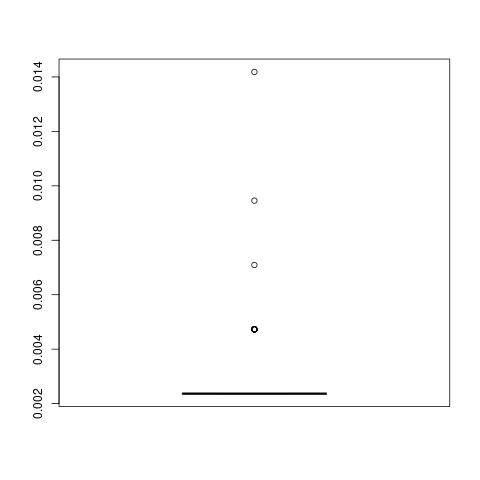
\includegraphics[width=0.32\textwidth]{Images/pv_pre/6h.png}
		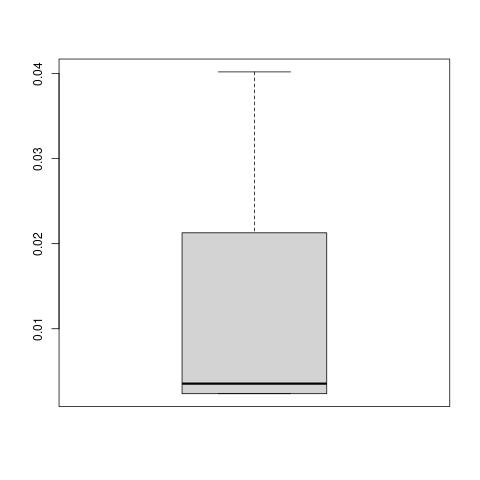
\includegraphics[width=0.32\textwidth]{Images/pv_pre/06:30:00.jpg}
		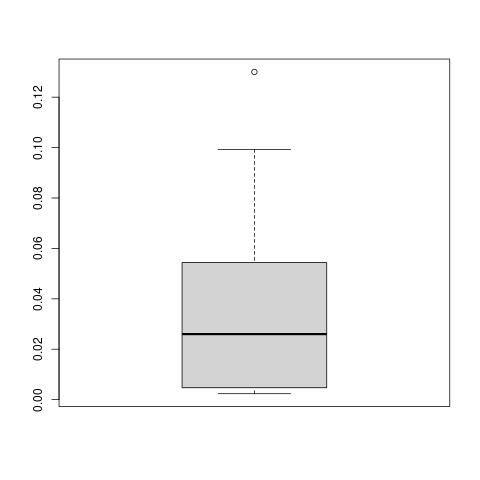
\includegraphics[width=0.32\textwidth]{Images/pv_pre/07:00:00.jpg}
	\end{minipage}
	\begin{minipage}{\linewidth}
		\centering
		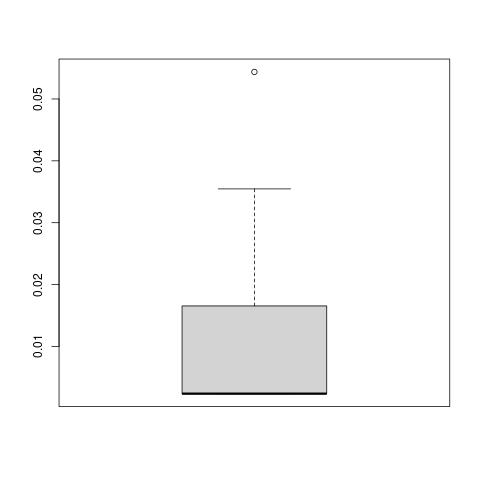
\includegraphics[width=0.32\textwidth]{Images/pv_pre/20:30:00.jpg}
		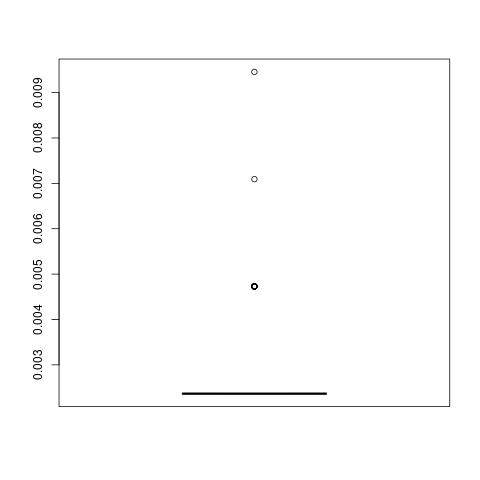
\includegraphics[width=0.32\textwidth]{Images/pv_pre/21:00:00.jpg}
		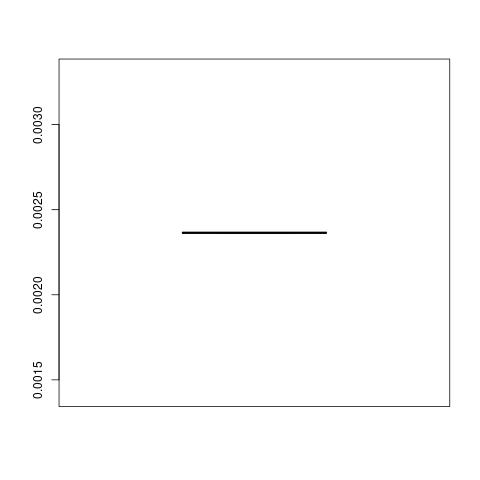
\includegraphics[width=0.32\textwidth]{Images/pv_pre/21:30:00.jpg}
	\end{minipage}
	\begin{minipage}{0.32\textwidth}
		\centering
		20h30
	\end{minipage}
	\begin{minipage}{0.32\textwidth}
		\centering
		21h
	\end{minipage}
	\begin{minipage}{0.32\textwidth}
		\centering
		21h30
	\end{minipage}
	\caption{Distribution du facteur de charge l'ensemble des journées d'un parc photovoltaïque pendant la période estivale, observée à différentes heures}
	\label{fig:boxplot_pv_journee}

	\smallskip

	\normalem

	\emph{On constate qu'avant 6h30 et après 20h30, la distribution de la production électrique est telle que l'on peut la considérer nulle : des valeurs extrêmes de l'ordre de grandeur de $10^{-3}$ en facteur de charge et très concentrées autour d'une valeur presque nulle. Pendant les périodes de jour ( entre 6h30 et 20h30 ) on observe un étalement dans la distribution ainsi que des valeurs plus élevées de l'odre de grandeur de $10^{-2}$ à $10^{-1}$ pour le début de la journée.}

\end{figure}
